\documentclass{article}
\usepackage{mainPoly}

\title{Chapitre 2 : Second degré}
\date{}
\author{Premières Spécialité Mathématiques}

\begin{document}
\maketitle

\section{Définition}

\begin{tcolorbox}
\begin{definition}
Une \textbf{fonction polynomiale du second degré} est une fonction $f$ définie sur les réels qui à tout nombre $x$ associe un réel $f(x)$ de la forme:
\begin{equation*}
ax^2+bx+c   
\end{equation*}
où $a$, $b$ et $c$ sont des réels avec $a \neq 0$. 
\end{definition}
\end{tcolorbox}
\begin{remark}
L'hypothèse $a \neq 0$ est essentielle, sinon la fonction est polynomiale de degré au plus $1$.    
\end{remark}
L'objectif de ce chapitre est d'étudier les fonctions polynomiales du second degré : l'allure de leur courbe représentative, leur extremum, leurs racines\dots
\section{Allure du graphique}
On trace la courbe représentative de deux fonctions polynomiales du second degré : une avec $a > 0$ et une avec $a < 0$.

\vspace*{1cm}
\begin{minipage}{0.45\textwidth}
\begin{center}
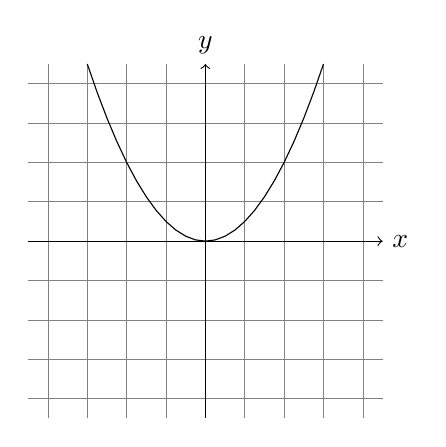
\begin{tikzpicture}
\draw[help lines] (-2.25,-2.25) grid[step=0.5] (2.25,2.25);
\draw[->] (-2.25,0) -- (2.25,0) node[right] {$x$};
\draw[->] (0,-2.25) -- (0,2.25) node[above] {$y$};
\draw[domain=-1.5:1.5] plot (\x, \x*\x);
\end{tikzpicture}
\end{center}   
\end{minipage}
\hfill
\begin{minipage}{0.45\textwidth}
\begin{center}
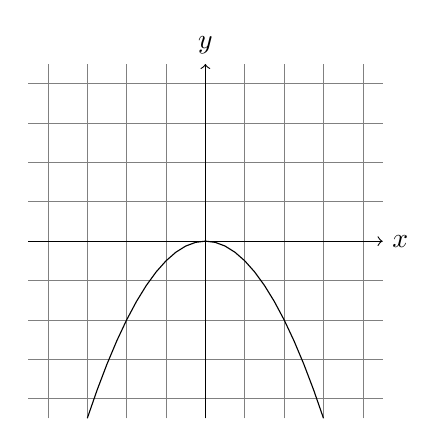
\begin{tikzpicture}
\draw[help lines] (-2.25,-2.25) grid[step=0.5] (2.25,2.25);
\draw[domain=-1.5:1.5] plot (\x, -\x*\x);
\draw[->] (-2.25,0) -- (2.25,0) node[right] {$x$};
\draw[->] (0,-2.25) -- (0,2.25) node[above] {$y$};
\end{tikzpicture}
\end{center}    
\end{minipage}
\vspace*{0.5cm}
\begin{tcolorbox}
\begin{definition}
Soit $f$ une fonction polynomiale de degré $2$. Sa courbe représentative est appelée une \textbf{parabole}.
\end{definition}
\end{tcolorbox}
\begin{proposition}
Soit $f$ une fonction polynomiale de degré $2$. telle que $f(x) = ax^2 + bx + c$. Alors:
\begin{itemize}
\item Si $a > 0$, il existe une valeur de $x$, notée $x_m$ telle que $f$ est décroissante sur $\left] - \infty; x_m \right]$ et croissante sur $\left[x_m; + \infty \right[$
\item Si $a < 0$, il existe une valeur de $x$, notée $x_M$ telle que $f$ est croissante sur $\left] - \infty; x_M \right]$ et décroissante sur $\left[x_M; + \infty \right[$
\end{itemize}
\end{proposition}
\begin{remark}
\hfill
\begin{itemize}
\item Dans le cas $a > 0$, les \emph{\og branches de la paraboles sont tournées vers le haut \fg}. Dans le cas contraire ($a < 0$), elles sont \emph{\og tournées vers le bas \fg}.
\item Dans le cas $a > 0$, $f$ admet un unique minimum, et ce minimum est atteint en $x_m$. Dans le cas contraire ($a < 0$), $f$ admet un maximum, et ce maximum est atteint en $x_M$. 
\end{itemize}
\end{remark}
\newpage
\section{Recherche de l'extremum}
\subsection{Forme canonique}
\begin{tcolorbox}
\begin{proposition}
Soit $f$ une fonction polynomiale du second degré telle que $f(x) = ax^2 + bx + c$. Alors il existe $\alpha$ et $\beta$ tel que
\begin{equation*}
f(x) = a(x - \alpha)^2 + \beta
\end{equation*}
\end{proposition}
\end{tcolorbox}
\emptybox{10cm}

\begin{remark}
Dans ce cas, $\alpha = \dfrac{-b}{2a}$ et $\beta = f(\alpha)$.
\end{remark}
\begin{example}
Soit l'expression polynomiale du second degré $- x^2 + 2x - 5$. Déterminer sa forme canonique.
\paragraph{Méthode 1}
Par identification :

\emptybox{3cm}
\paragraph{Méthode 2} En utilisant les \og presque \fg identités remarquables :

\emptybox{3cm}
\end{example}
\newpage
\subsection{Extremum}
\begin{tcolorbox}    
\begin{proposition}
Soit une fonction polynomiale du second degré $f : x \mapsto ax^2 + bx + c$. On suppose que $f(x) = a(x - \alpha)^2 + \beta$ pour tout $x$ réel. Alors, $f$ admet un extremum qu'il atteint en $\alpha$ et ayant pour valeur $\beta$.    
\end{proposition}
\end{tcolorbox}
    \begin{remark}
Comme dit précédemment, si $a > 0$, alors $f$ admet un minimum qu'il attent en $\alpha = \dfrac{-b}{2a}$. Sinon, si $a < 0$, alors $f$ admet un maximum qu'il atteint en $\alpha = \dfrac{-b}{2a}$. Dans les deux cas, cet extremum vaut $\beta = f(\alpha)$.
\end{remark}
\begin{example}
Soit la fonction polynomiale $g : x \mapsto 4x^2 + 32x - 5$.
\begin{enumquestions}
\item Cette fonction admet-elle un minimum ou un maximum ?
\item En quelle valeur cet extremum est-il atteint ?
\item Que vaut cet extremum ?
\end{enumquestions}
\emptybox{5cm}
\end{example}
\begin{proposition}
Soit $f : x \mapsto ax^2 + bx + c$ une fonction polynomiale du second degré. On suppose que $f(x) = a(x - \alpha)^2 + \beta$. Alors la courbe représentative $\mathcal{C}_f$ est une parabole admettant comme axe de symétrie la droite $x = \alpha$.
\end{proposition}
\begin{example}
Soit $f : x \mapsto x^2 - 2x + 1$. Alors $f$ admet un minimum (car $a > 0$) atteint en $\alpha = - \dfrac{b}{2a} = - \dfrac{-2}{2} = 1$. Alors $\mathcal{C}_f$ admet la droite $x = 1$ comme axe de symétrie.
\begin{center}
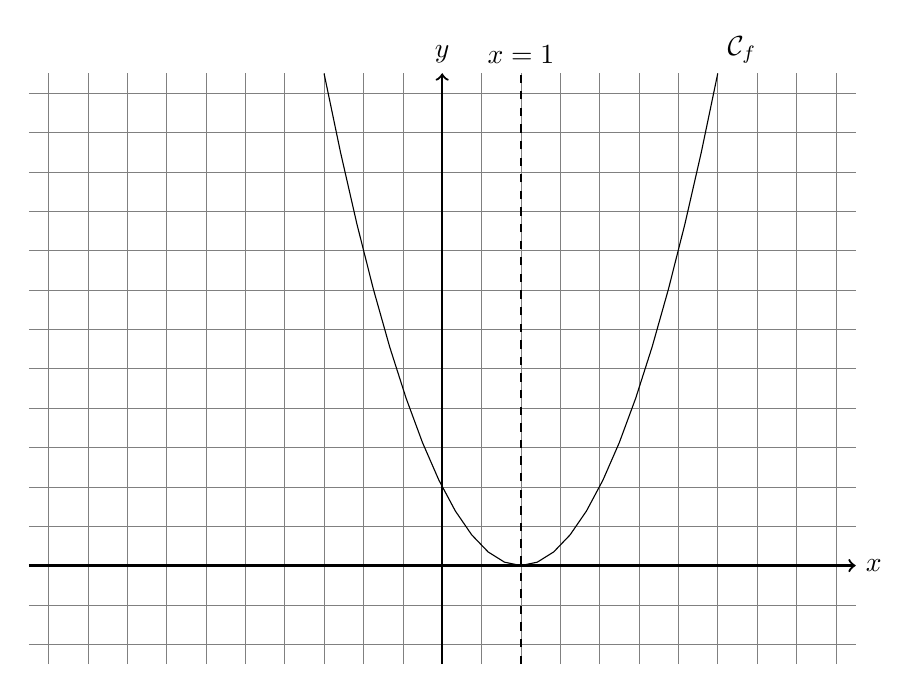
\begin{tikzpicture}
\draw[help lines] (-5.25,-1.25) grid[step=0.5] (5.25,6.25);
\draw[->,thick] (-5.25,0) -- (5.25,0) node[right] {$x$};
\draw[->,thick] (0,-1.25) -- (0,6.25) node[above] {$y$};
\draw plot[domain=-1.5:3.5] (\x, \x * \x - 2 * \x + 1) node[above right] {$\mathcal{C}_f$};
\draw[dashed,thick] (1,-1.25) -- (1,6.25) node[above] {$x = 1$};
\end{tikzpicture}
\end{center}
\end{example}

\newpage

\section{Racines}

\subsection{Définition}

\begin{tcolorbox}
\begin{definition}
Soit $f$ une fonction. On appelle \textbf{racine} de la fonction $f$ un nombre $r$ tel que $f(r) = 0$.
\end{definition}
\end{tcolorbox}
\begin{example}
Montrer que $r_1 = 1$ et $r_2 = - 3$ sont deux racines de la fonction $f : x \mapsto 2x^2 + 4x - 6$.

\emptybox{3cm}
\end{example}
\end{document}